\documentclass[a4paper,11pt]{article}

%\usepackage{german}

\usepackage[dvipsnames]{xcolor}
\usepackage{graphicx}

\usepackage{amssymb}

\usepackage{amsfonts}

\usepackage{amsmath}

\usepackage{amsthm}

\usepackage[unicode=true, pdfusetitle, bookmarks=true,
  bookmarksnumbered=false, bookmarksopen=false, breaklinks=true, 
  pdfborder={0 0 0}, backref=false, colorlinks=true, linkcolor=blue,
  citecolor=blue, urlcolor=blue]{hyperref}
\usepackage{slashed}
\usepackage{authblk}
%identity sign
\usepackage{dsfont}

\usepackage{relsize}




\DeclareMathOperator{\tr}{tr}


%commutative diagrams
\usepackage{amsmath,amscd}


\addtolength{\textwidth}{2.2cm} \addtolength{\hoffset}{-1.0cm}

\addtolength{\textheight}{3.0cm} \addtolength{\voffset}{-2cm} 

\parindent 0cm

\pagestyle{empty}

\begin{document}
\title{Regularity of high orders}

%\author{}

\date{\today}



\maketitle

\section{modified Bessel functions}

In these calculations the modified Bessel function of the second kind and first order \(K_1\) plays repeatedly a big role. 
Here are some properties of it. There are several integral representations of it, the first two are especially compact expressions, 
whereas the \href{https://dlmf.nist.gov/10.32#E14}{last one} has a very large domain of validity  :

\begin{multline}\label{defK}
K_1(\xi) = \xi \int_1^\infty e^{-\xi s} \sqrt{s^2-1} ds = \int_0^\infty e^{-\xi \sqrt{1+s^2}} ds \\
=\frac{i e^{-\xi}}{(2\pi)^{\frac{3}{2}} \sqrt{x}} \int_{- i \infty}^{i \infty} \Gamma(s) \Gamma\left( - \frac{1}{2} - s\right) \Gamma \left( \frac{1}{2}-s\right) (2\xi)^{s} ds,
\end{multline}
please note that 
\begin{equation}
\left|\Gamma(i s) \Gamma\left( - \frac{1}{2} - i s\right) \Gamma \left( \frac{1}{2}-i s\right)\right| = 9 ~\pi^{\frac{3}{2}} \frac{\left(\frac{1}{4} + s^2\right)^2}{\sqrt{s \sinh (\pi s)} \cosh( \pi s)} ~~ \forall s \in \mathbb{R},
\end{equation}
holds which makes the last integral convergent whenever \(|\text{arg } \xi|<\frac{3}{2}\pi\). Please also take note that the integral contour of the last expression is nontrivial, it separates the poles of \(\Gamma(s)\) from the poles of the other two \(\Gamma\) functions like this:

%\begin{wrapfigure}{L}{0.45\textwidth}
%\centering
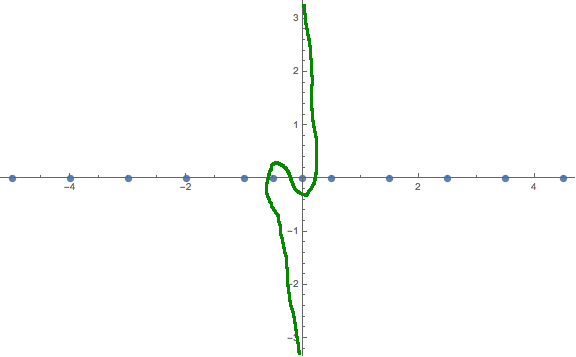
\includegraphics[width=0.7\textwidth]{GammaPolesContour}
%\caption{\label{fig:dirac_sea}contour of integration}
%\end{wrapfigure}

The function \(K_1\)can be expanded in a series in the logarithm like this

\begin{equation}\label{K1series}
K_1(\xi) = \frac{1}{\xi}- \frac{\xi}{4} \sum_{k=0}^\infty \left(2 \psi(k+1)+\frac{1}{k+1}-2 \ln\frac{ \xi}{2} \right) \frac{\left(\frac{\xi^2}{4}\right)^k}{k!^2 (k+1)},
\end{equation}

where

\begin{equation}
\forall n \in \mathbb{N}:~~\psi(n)= -\gamma + \sum_{l=1}^{n-1} l^{-1} 
\end{equation}

is the digamma function for positive integer arguments and \(\gamma\) is the Euler-Mascheroni constant.

\section{Projector onto the Negative Energy Subspace}

For \(\phi,\xi \in \mathcal{H}_\Sigma\) we define the action of the projector on \(\Sigma\) to be

\begin{equation}
\langle \phi, P^-_\Sigma \xi\rangle = \lim_{\varepsilon \searrow 0} \int_{x \in \Sigma} \overline{\phi}(x) i_\gamma (d^4x)
\int_{y \in \Sigma} p^-(y-x+i \varepsilon u)) i_\gamma(d^4 y) \xi (y),
\end{equation}

where \(u\) is some arbitrary fixed time like vector pointing into the past and the kernel of \(P^-\) is given by

\begin{align}
p^-: \mathbb{R}^4+i \text{Past} \rightarrow \mathbb{C}^{4\times 4}, p^-(w) = \frac{1}{(2\pi)^3 m}\int_{\mathcal{M}^-}\frac{\slashed{p} +m}{2m}e^{i pw}i_p(d^4p) = \frac{-i \slashed{\partial}+m}{2m}D(w),\\
D:\mathbb{R}^4+ i \text{Past}\rightarrow \mathbb{C}, D(w)= \frac{1}{(2\pi)^3 m} \int_{\mathcal{M}^-}e^{i pw} i_p(d^4p) = -\frac{m^3}{2\pi^2}\frac{K_1(m \sqrt{-w^2})}{m \sqrt{-w^2}}.
\end{align}

The square in the last equation denotes \(w^2=\sum_{\alpha=0}^3 w^\alpha w_\alpha\).


\section{Greens Functions}


The Greens functions of the Klein-Gordon \(D_\pm\) equation is defined by the equation

\begin{equation}
(\square +m^2) D_\pm (x)=\delta^4(x).
\end{equation}

From this equation and the condition on the support of the advanced/retarded Greens function \(\text{supp} D_\pm \subseteq \{x\in \mathbb{R}^4\mid  \pm x^0\ge 0\}\) it follows that 

\begin{equation}
D_\pm (x)= \frac{1}{(2\pi)^4} \int_{\mathbb{R}^4\pm i \varepsilon e_0}d^4p \frac{1}{m^2-p^2} e^{-i p x}
\end{equation}

holds, where \(\varepsilon>0\) is arbitrary. From the identity \((i\slashed{\partial} -m)(-i \slashed{\partial} -m)=\square +m^2\) we can directly
infer the Fourier representation of the Greens function of the Dirac equation, namely

\begin{multline}
\Delta_\pm (x)= -(i\slashed{\partial} +m) D_\pm (x)
=\frac{1}{(2\pi)^4} \int_{\mathbb{R}^4 \pm i \varepsilon e_0}d^4p \frac{\slashed{p}+m}{p^2-m^2}e^{-i p x}\\
=\frac{1}{(2\pi)^4} \int_{\mathbb{R}^4 \pm i \varepsilon e_0}d^4p (\slashed{p}-m)^{-1}e^{-i p x}.
\end{multline}

As a consistency check we verify \(i (\Delta_+-\Delta_-)=P^++P^-\) (for a justification of that factor of \(i\) 
see appendix \ref{AppendixPropagatorGreens}):

\begin{align}
\Delta_+-\Delta_-=\frac{i\slashed{\partial} +m}{(2\pi)^4}\left(\int_{\mathbb{R}^4+i\varepsilon e_0}d^4p \frac{e^{-ipx}}{p^2-m^2} -\int_{\mathbb{R}^4-i\varepsilon e_0}d^4p \frac{e^{-ipx}}{p^2-m^2} \right)\\
=\frac{i\slashed{\partial} +m}{(2\pi)^4} \int_{\raisebox{-15pt}{$\overset{\xrightarrow{~~~~~~~}}{\xleftarrow{~~\cdot~\cdot~~}}$}}d^4 p \frac{e^{-ipx}}{p^2-m^2}
=\frac{i\slashed{\partial} +m}{(2\pi)^4} \int_{\mathlarger{\circlearrowright} \!\!\!\!\raisebox{0.3pt}{$\cdot$}~\mathlarger{\circlearrowright} \!\!\!\!\raisebox{0.3pt}{$\cdot$}} d^4 p \frac{e^{-ipx}}{(p^0+E(\vec{p}))(p^0-E(\vec{p}))}\\
=-2\pi i \frac{i\slashed{\partial} +m}{(2\pi)^4}\left( \int_{\mathbb{R}^3}\left. \frac{e^3p e^{-ipx}}{-2E(\vec{p})}\right|_{p^0=-E(\vec{p})} +\int_{\mathbb{R}^3}\left. \frac{e^3 p e^{-ipx}}{2E(\vec{p})}\right|_{p^0=E(\vec{p})} \right)\\
=\frac{-i}{(2\pi)^3m} \frac{(i \slashed{\partial}+m)}{2m}\left(\int_{\mathbb{R}^3} \left.\frac{m^2 d^3 p  e^{-ipx}}{-E(\vec{p})}\right|_{p^0=-E(\vec{p})}+\int_{\mathbb{R}^3} \left.\frac{m^2 d^3 p e^{-ipx}}{E(\vec{p})}\right|_{p^0=E(\vec{p})}\right)\\
=\frac{-i}{(2\pi)^3m} \frac{i \slashed{\partial}+m}{2m} \left( \int_{\mathcal{M}^-}i_p(d^4p) e^{-ipx} + \int_{\mathcal{M}^+}i_p(d^4p) e^{-ipx}\right)=-i (P^-+P^+).
\end{align}

\subsection{Explicit Representation of Greens Functions}

Now since we will work with these Greens functions, we would like to have a more explicit spacetime representation. 
For this purpose let \(x^0>0\) and let \(f\in C_c^\infty (\mathbb{R}^3)\), we compute

\begin{align}
\int_{\mathbb{R}^3} D_\pm (x) f(\vec{x})d^3x = \frac{-1}{(2\pi)^4} \int_{\mathbb{R}^4\pm i \varepsilon e_0} d^4p \frac{e^{-ip^0 x^0}}{p^2-m^2} \int_{\mathbb{R}^3} d^3x e^{i\vec{p}\cdot \vec{x}} f(\vec{x})\\
=\frac{-1}{(2\pi)^{\frac{5}{2}}} \int_{\mathbb{R}^4\pm i \varepsilon e_0} d^4p \frac{e^{-ix^0 p^0}}{p^2-m^2}\hat{f}(\vec{p})\\
=\frac{-1}{(2\pi)^{\frac{5}{2}}} \int_{\mathbb{R}^3} d^3p \int_{\mathbb{R}\pm i \varepsilon}dp^0 \frac{e^{-ix^0 p^0}}{(p^0-E(\vec{p}))(p^0+E(\vec{p}))}\hat{f}(\vec{p})\\\label{time sign change}
\overset{*}{=}\frac{-1}{(2\pi)^{\frac{5}{2}}}  \left\{\begin{matrix}D_+:&&~ \int_{\mathbb{R}^3}d^3p  (-2\pi i)\left(\frac{e^{-ix^0 E(\vec{p})}}{2E(\vec{p})}+\frac{e^{ix^0 E(\vec{p})}}{-2E(\vec{p})} \right) \hat{f}(\vec{p})
\\D_-:&& 0 \end{matrix} \right.\\
=\frac{1}{(2\pi)^{\frac{3}{2}}} \int_{\mathbb{R}^3} d^3p\left\{ \begin{matrix}D_+: &&\sin(E(\vec{p})x^0)\\D_-:  &&0 \end{matrix}\right\} \hat{f}(\vec{p}).
\end{align}

where for the with \(*\) marked equality we closed the contour in the lower half plane, enclosing no pole for \(D_-\) while enclosing both
poles for \(D_+\). We will further analyse the expression obtained for \(D_+\), first since \(\hat{f}\) decays 
fast enough for large arguments we can introduce 
the following limit via Lebesgues theorem of dominated convergence:

\begin{align}
\int_{\mathbb{R}^3} D_+ (x) f(\vec{x})d^3x =\frac{-2i}{(2\pi)^{\frac{3}{2}}} \lim_{\varepsilon \searrow 0}\int_{\mathbb{R}^3} d^3p
\left( \frac{e^{i (x^0+i \varepsilon) E(\vec{p})}}{E(\vec{p})} - \frac{e^{-i (x^0-i \varepsilon)E(\vec{p})}}{E(\vec{p})} \right) \hat{f}(\vec{p})\\
\overset{*}{=} \frac{-2i}{(2\pi)^{3}} \lim_{\varepsilon \searrow 0}  \int_{\mathbb{R}^3} d^3 x \int_{\mathbb{R}^3} d^3 p 
\left( \frac{e^{i E(\vec{p})(x^0+i\varepsilon)}}{E(\vec{p})} 
-\frac{e^{-i E(\vec{p})(x^0-i\varepsilon)}}{E(\vec{p})} \right)e^{i\vec{p}\cdot \vec{x}}f(\vec{x}),
\end{align}

where for the marked equality we used the theorem of Plancherel. Now we look at one of the summands in the inner integral

\begin{align}
\int_{\mathbb{R}^3}d^3p \frac{e^{iE(\vec{p})(x^0+i\varepsilon)}}{E(\vec{p})} e^{i\vec{p}\cdot\vec{x}} \\
= 2\pi \int_0^\infty dp \frac{p^2}{\sqrt{m^2+p^2}} e^{i \sqrt{m^2+p^2}(x^0+i\varepsilon)} \int_{-1}^1 d \cos \theta e^{i p |\vec{x}| \cos \theta}\\
=2\pi \int_0^\infty dp \frac{p^2}{\sqrt{m^2+p^2}} e^{i \sqrt{m^2+p^2}(x^0+i\varepsilon)} \frac{1}{i p |\vec{x}} \left(e^{i p |\vec{x}|} - e^{-i p |\vec{x}|}\right)\\
=4\frac{\pi}{|\vec{x}|} \int_0^\infty dp \frac{p}{\sqrt{m^2+p^2}} e^{i \sqrt{m^2+p^2}(x^0+i\varepsilon)} \sin( p |\vec{x}|)\\
\overset{\text{Gradsteyn, Ryzhik}, 3.961.1}{=} 4\pi m^2 \frac{K_1\left(m \sqrt{|\vec{x}|^2 + (\varepsilon - i x_0)^2}\right)}{m \sqrt{|\vec{x}|^2 + (\varepsilon - i x_0)^2}}
\end{align}

Analogously the second summand yields 

\begin{equation}
-\int_{\mathbb{R}^3}d^3p \frac{e^{-i(x^0-i\varepsilon)E(\vec{p})}}{E(\vec{p})}= -m^2 4 \pi \frac{K_1\left( m \sqrt{(\varepsilon + i x^0)^2+\vec{x}^2}\right)}{ m \sqrt{(\varepsilon + i x^0)^2+\vec{x}^2}},
\end{equation}

putting the last three calculations together we find an explicit expression of the action of \(D_+\)
for \(x^0>0\):

\begin{align}
\int_{\mathbb{R}^3} D_+(x)f(\vec{x})d^3x= \frac{-2i}{(2\pi)^3} \lim_{\varepsilon \searrow 0} \int_{\mathbb{R}^3} d^3 x  m^2 4\pi \\
\left(\frac{K_1\left(m \sqrt{|\vec{x}|^2 + (\varepsilon - i x_0)^2}\right)}{m \sqrt{|\vec{x}|^2 + (\varepsilon - i x_0)^2}}
-\frac{K_1\left(m \sqrt{|\vec{x}|^2 + (\varepsilon + i x_0)^2}\right)}{m \sqrt{|\vec{x}|^2 + (\varepsilon + i x_0)^2}}
  \right) f(\vec{x})\\
  =\frac{2 m^2}{\pi^2} \lim_{\varepsilon \searrow 0} \int_{\mathbb{R}^3} d^3x \Im\left( \frac{K_1\left(m \sqrt{|\vec{x}|^2 + (\varepsilon - i x_0)^2}\right)}{m \sqrt{|\vec{x}|^2 + (\varepsilon - i x_0)^2}}
  \right) f(\vec{x}).
  \end{align}


For \(x^0<0\) the same calculation can be done with the only difference being that the contour in \eqref{time sign change} is closed in
upper half plane, which means that the contribution of \(D_+\) vanishes while for the one for \(D_-\) the contour has 
a positive winding number of 1 instead of one of -1. Doing this results in 

\begin{align}
\int_{\mathbb{R}^3} D_-(x)f(\vec{x})d^3x
  =\frac{2 m^2}{\pi^2} \lim_{\varepsilon \searrow 0} \int_{\mathbb{R}^3} d^3x \Im\left( \frac{K_1\left(m \sqrt{|\vec{x}|^2 + (\varepsilon + i x_0)^2}\right)}{m \sqrt{|\vec{x}|^2 + (\varepsilon + i x_0)^2}}
  \right) f(\vec{x}).
  \end{align}

Lastly the \(x^0=0\) case can be integrated directly,

\begin{align}
\int_{\mathbb{R}^3} D_{\pm}(x) f(\vec{x})
=\frac{-1}{(2\pi)^{\frac{5}{2}}} \int_{\mathbb{R}^3} d^3p \int_{\mathbb{R}\pm i \varepsilon}dp^0 \frac{1}{(p^0-E(\vec{p}))(p^0+E(\vec{p}))}\hat{f}(\vec{p})
\end{align}

here we evaluate the inner integral:

\begin{align}
\int_{\mathbb{R}\pm i \varepsilon}dp^0 \frac{1}{(p^0-E(\vec{p}))(p^0+E(\vec{p}))}=
\int_{\mathbb{R}}dp^0 \frac{1}{(p^0\pm i \varepsilon-E(\vec{p}))(p^0\pm i \varepsilon+E(\vec{p}))}=\\
\int_\mathbb{R} dp^0 \frac{1}{2 E(p)} \left( \frac{1}{p^0\pm i \varepsilon -E(p)} - \frac{1}{p^0 \pm i \varepsilon + E(p)}\right)=\\
\frac{1}{2E(p)} \left.\left( \ln (p^0\pm i\varepsilon -E(p)) - \ln (p^0 \pm i \varepsilon + E(p))\right)\right|_{p^0=-\infty}^\infty=\\
\frac{1}{2E(p)} \left.\left( \ln\frac{ p^0\pm i\varepsilon -E(p)}{p^0 \pm i \varepsilon + E(p)}\right)\right|_{p^0=-\infty}^\infty=0.
\end{align}


Summarising we write for general \(x^0\in \mathbb{R}\)

\begin{equation}\label{ImK1}
\int_{\mathbb{R}^3}d^3 x D_\pm (x) f(\vec{x}) = 
\mp \theta_0(\pm x^0) \frac{2 m^2}{\pi^2} \lim_{\varepsilon \searrow 0} \int_{\mathbb{R}^3}d^3 x f(\vec{x}) \Im 
\frac{K_1(m \sqrt{-x^2 +2 i \varepsilon x^0 + \varepsilon^2})}{m \sqrt{-x^2 +2 i \varepsilon x^0 + \varepsilon^2}},
\end{equation}

where \(\theta_0(y)=\left\{\begin{matrix} 1 && y>0 \\ 0 && y\le 0 \end{matrix} \right.\) is a version of the Heavyside function.

\subsection{Taking the Limit}

In order to further evaluate \eqref{ImK1} we are going to split \(\frac{K_1(\sqrt{\cdot})}{\sqrt{\cdot}}\) up into three parts. 
Starting with the series \eqref{K1series} we split the part involving the logarithm up:

\begin{align}
\frac{K_1(\sqrt{\xi})}{\sqrt{\xi}}=\frac{1}{\xi} +   \overbrace{\frac{1}{4}\sum_{k=0}^\infty \frac{\xi^k}{4^k k!^2 (k+1)}}^{=:I(\xi)} \ln \frac{\xi}{4}
-\frac{1}{4}\sum_{k=0}^\infty \left(2\psi(k+1) + \frac{1}{k+1}\right) \frac{\xi^k}{4^k k!^2 (k+1)},
\end{align}

where \(I\) is entire and real on the real line, which is also true about the last term.
Let \(x^0\neq 0\) and \(f\in C_c^\infty(\mathbb{R}^3)\) as before, 
we are going to massage the first part of the right hand side of \eqref{ImK1}, which is

\begin{align}
\mp \theta_0(\pm x^0) \frac{2 m^2}{\pi^2} \lim_{\varepsilon \searrow 0} \int_{\mathbb{R}^3} d^3x f(\vec{x}) \Im \frac{1}{m^2 (-x^2 + 2 i \varepsilon x^0 + \varepsilon^2)}\\
=\mp \theta_0(\pm x^0) \frac{2 }{\pi^2} \lim_{\varepsilon \searrow 0}\int_0^\infty dy  \overbrace{\int_{S^2} d\Omega f(\Omega, y) y^2}^{=:g(y)} \Im \frac{1}{-(x^0)^2+ y^2 + 2 i \varepsilon x^0 + \varepsilon^2}\\
=\mp \theta_0(\pm x^0) \frac{2 }{\pi^2} \lim_{\varepsilon \searrow 0}\int_0^\infty dy~ g(y)\frac{1}{2\sqrt{(x^0)^2-i \varepsilon x^0 - \varepsilon^2}} \\
\Im 
 \Big(\frac{1}{y+ \sqrt{(x^0)^2-2 i \varepsilon x^0 - \varepsilon^2}}-\frac{1}{y- \sqrt{(x^0)^2-2 i \varepsilon x^0 - \varepsilon^2}} \Big)\\
=\mp \theta_0(\pm x^0) \frac{1 }{|x^0|\pi^2} 
 \Big(\lim_{\varepsilon \searrow 0}\int_0^\infty dy~ g(y) \Im \frac{1}{y+ \sqrt{(x^0)^2-2 i \varepsilon x^0 - \varepsilon^2}}\\
-\lim_{\varepsilon \searrow 0}\int_0^\infty dy~ g(y) \Im \frac{1}{y- \underbrace{\sqrt{(x^0)^2-2 i \varepsilon x^0 - \varepsilon^2}}_{:= \alpha_\varepsilon + i \beta_\varepsilon}}\Big)\\
\overset{\text{Lebesgue d.c.}}{=}\mp \theta_0(\pm x^0) \frac{1 }{|x^0|\pi^2} 
 \left(\int_0^\infty dy~ g(y) \Im \frac{1}{y+|x^0|}\right.\\
\left.-\lim_{\varepsilon \searrow 0}\int_0^\infty dy~ g(y) \Im \frac{1}{y- \alpha_\varepsilon -i \beta_\varepsilon}\right)\\
=\mp \theta_0(\pm x^0) \frac{-1 }{|x^0|\pi^2} \lim_{\varepsilon \searrow 0} \int_0^\infty dy g(y) \frac{\beta_\varepsilon}{(y-\alpha_\varepsilon)^2+\beta_\varepsilon^2}\\
\overset{|\beta_\varepsilon|(z-\alpha_\varepsilon) :=y}{=}\mp \theta_0(\pm x^0) \frac{-1 }{|x^0|\pi^2} 
\lim_{\varepsilon \searrow 0} \int_{-\frac{\alpha_\varepsilon}{|\beta_\varepsilon|}}^\infty dz 
 g(z |\beta_\varepsilon|+\alpha_\varepsilon) \text{sgn}(\beta_\varepsilon) \frac{1}{ z^2+1}\\
 \overset{\text{Lebesuge d.c.}}{=}\mp \theta_0(\pm x^0) \frac{-1 }{|x^0|\pi^2} 
\int_\mathbb{R} dz\frac{1}{z^2+1}\lim_{\varepsilon \searrow 0}  1_{z>-\frac{\alpha_\varepsilon}{|\beta_\varepsilon|}} g(z |\beta_\varepsilon|+\alpha_\varepsilon) \text{sgn}(\beta_\varepsilon)\\
=\mp \theta_0(\pm x^0) \frac{-1 }{|x^0|\pi^2} \int_\mathbb{R} dz\frac{1}{z^2+1}  g(|x^0|) \text{sgn}(- x^0)\\
=\mp \theta_0(\pm x^0) \frac{\text{sgn}(x^0)}{|x^0| \pi} g(|x^0|)\\
=\mp \theta_0(\pm x^0) \frac{\text{sgn}(x^0)}{|x^0| \pi} \int_{S^2} d\Omega |x^0|^2 f(\Omega, |x^0|)\\
=\mp \theta_0(\pm x^0) \frac{2~\text{sgn}(x^0)}{ \pi} \int_{\mathbb{R}^3} d^3x \delta(x^2) f(\vec{x}).
\end{align}

Next up is the part proportional to a logarithm, we will use the same abbreviation \(g\),

\begin{align}
\mp \theta_0(\pm x^0) \frac{2m^2}{\pi^2} \lim_{\varepsilon \searrow 0} \int_{\mathbb{R}^3} d^3x f(\vec{x})~~~~~~~~~~~~~~~~~~~~~~~~~~~~~~~~~~~~~~~~~~~~~\\
 \Im \ln \overbrace{\frac{m^2(-x^2+2i\varepsilon x^0 + \varepsilon^2)}{4} }^{=: r_\varepsilon (|\vec{x}|)e^{i \varphi_\varepsilon (|\vec{x}|)}}I(m^2 (-x^2+2i\varepsilon x^0 + \varepsilon^2))\\
=\mp \theta_0(\pm x^0) \frac{2m^2}{\pi^2} \lim_{\varepsilon \searrow 0} \int_\mathbb{R} dy g(y) \Im \Big[\ln r_\varepsilon(y)
I(m^2 (-(x^0)^2 + y^2+2i\varepsilon x^0 + \varepsilon^2))\Big]\\
\mp \theta_0(\pm x^0) \frac{2m^2}{\pi^2} \lim_{\varepsilon \searrow 0} \int_\mathbb{R} dy g(y) \Im\Big[ i \varphi_\varepsilon(y)
 I(m^2 (-(x^0)^2 + y^2+2i\varepsilon x^0 + \varepsilon^2))\Big]\\
 \overset{\text{Lebesgue d.c.}}{=}\mp \theta_0(\pm x^0) \frac{2m^2}{\pi^2}  \int_\mathbb{R} dy g(y) \Im \Big[\ln |(x^0)^2-y^2|
I(m^2 (-(x^0)^2 + y^2))\Big]\\
\mp \theta_0(\pm x^0) \frac{2m^2}{\pi^2}  \int_\mathbb{R} dy g(y)\lim_{\varepsilon \searrow 0} \Im[ i \varphi_\varepsilon(y)]
 I(m^2 (-(x^0)^2 + y^2))\\
 =\mp \theta_0(\pm x^0) \frac{2m^2}{\pi^2}  \int_\mathbb{R} dy g(y) \pi \text{sgn}(x^0) \theta((x^0)^2-y^2)
 I(m^2 (-(x^0)^2 + y^2))\\
 = \mp \theta_0(\pm x^0) \frac{2 m^2}{\pi} \int_{\mathbb{R}^3} d^3 x f(\vec{x}) \text{sgn}(x^0) \theta(x^2) I(-m^2x^2).
\end{align}

Now the last term in \(\frac{K_1(\sqrt{\cdot})}{\sqrt{\cdot}}\) is entire (therefore continuous on all of \(\mathbb{C}\)) 
and real on the real line, so by the same arguments which were used
in the last calculation this term does not survive Lebesgues dominated convergence and taking the imaginary Part. 
So we can give representation of \(D_\pm\) without a limit

\begin{align}
\int_{\mathbb{R}^3}d^3 x D_\pm (x) f(\vec{x}) = \mp \theta_0(\pm x^0)\frac{2 ~\text{sgn}(x^0)}{\pi} \int_{\mathbb{R}^3}d^3 x ( \delta(x^2)+m^2 \theta(x^2) I(-m^2x^2))f(\vec{x})\\
=- \theta_0(\pm x^0)\frac{2 }{\pi} \int_{\mathbb{R}^3}d^3 x ( \delta(x^2)+m^2 \theta(x^2) I(-m^2x^2))f(\vec{x}),
\end{align}

or in other words, the equation

\begin{equation}
D_\pm (x)=- \theta_0(\pm x^0)\frac{2 }{\pi} \left( \delta(x^2)+m^2 \theta(x^2) I(-m^2x^2)\right)
\end{equation}
holds.



\section{Expansion}
We would like to see whether high orders of the expansion of 


\begin{equation}\label{trace}
c_A(F,G)=\frac{1}{2} \partial_F \partial_G \tr \left[ P_- S_{A,A+G} P_+ S_{A,A+F} P_- - P_- S_{A,A+F} P_+ S_{A,A+G} P_- \right]
\end{equation}

is regular enough, so that we don't have to be worries about splitting the trace into the two summands and working with them separately.

From phase.tex we know that

\begin{equation}\label{SSeries}
\partial_F S_{A,A+F}= \Delta (1-\slashed{A}\Delta_-)^{-1} \slashed{F} ( 1-\Delta_+ \slashed{A})^{-1}
\end{equation}
holds. So it boils down to knowing how the regularity of a distribution \(H\) compares to the regularity of

\begin{equation}
\Delta_{\pm} * \slashed{A} H
\end{equation}

and 

\begin{equation}
 H \slashed{A} * \Delta_{\pm}.
\end{equation}

\subsection{Simple Convolutions}

Considering \eqref{trace} together with \eqref{SSeries} we are going to look at pieces which are going to make up the series. Starting at the
 operator product in one summand on the right we consider  \(\Delta_+ *(\slashed{A} P^-)\). Let therefore \(f_1,f_2 \in \mathcal{H}_\Sigma\) 
for some space-like hypersurface \(\Sigma\). The distribution in question evaluated at \(f_1, f_2\) yields

\begin{align}
&\langle f_1, \Delta_+ * (\slashed{A} P^- f_2)\rangle =\\
&\lim_{\varepsilon \searrow 0}\int_{\Sigma_x} \overline{f}_1(x) i_\gamma(d^4 x) \int_{\mathbb{R}^4}d^4y \Delta_+ (y-x)  \int_{\Sigma_z} \slashed{A}(y) p^-(z-y - i \varepsilon u) i_\gamma(d^4z) f_2(z),
\end{align}

now in order to study regularity of the involved distribution we start with the most singular parts of \(\Delta_+\) and \(P^-\), 
which are \(\frac{-2}{\pi}(-i\slashed{\partial}+m)\theta_0(\cdot^0)  \delta(\cdot^2)\) 
and \(\frac{1}{4 \pi}(-i\slashed{\partial}+m) \text{sgn}(\cdot^0) \delta(\cdot^2) + P_V ?\) respectively. 
We start with the convolution of the two derivatives of delta distributions: \textcolor{red}{geht partiall integrieren mit \(\gamma\)-Matrizen mit dem \(i_\gamma\) Maß genauso wie mit \(\gamma^0 d^3 x\) ?}

\begin{align}
\frac{-1}{2 \pi^2}\int_{\Sigma_x} \overline{f}_1(x) i_\gamma(d^4 x) 
\int_{\mathbb{R}^4}d^4y (i\slashed{\partial}_x+m)\theta_0(y^0-x^0)  \delta((y-x)^2) 
\\ \int_{\Sigma_z} \slashed{A}(y) (-i\slashed{\partial}_z+m) \text{sgn}(z^0-y^0) \delta((z-y)^2) i_\gamma(d^4z) f_2(z)\\
=\frac{-1}{2 \pi^2}\int_{\Sigma_x} \overline{(i\slashed{\partial}+m)f}_1(x) i_\gamma(d^4 x) 
\int_{\mathbb{R}^4}d^4y \theta_0(y^0-x^0)  \delta((y-x)^2)\\ 
\int_{\Sigma_z} \slashed{A}(y)  \text{sgn}(z^0-y^0) \delta((z-y)^2) i_\gamma(d^4z) (-i\slashed{\partial}+m) f_2(z).
\end{align}

Clearly the relevant integral to evaluate is the \(y\)-integral in the centre. We try to come as close as possible to this, we
start by writing out the delta distribution as a sum of the nodes of its argument

\begin{align}
\int_{\mathbb{R}^4} d^4 y~ \theta_0(y^0-x^0) \delta((y-x)^2) \text{sgn}(z^0-y^0) \delta((y-z)^2) \slashed{A}(y) \\
=\int_{\mathbb{R}^4} d^4 y~
 \frac{\delta(y^0-x^0 - |\vec{y}-\vec{x}|)}{2|\vec{y}-\vec{x}|}
\left( \frac{\delta(y^0-z^0 + |\vec{y}-\vec{z}|)}{2|\vec{y}-\vec{z}|} - \frac{\delta(y^0-z^0 - |\vec{y}-\vec{z}|)}{2|\vec{y}-\vec{z}|} \right)
\slashed{A}(y) .
\end{align}

Next in order to abbreviate things, we shift \(y\) by \(x\) and introduce \(w:= x-z\) while using the delta distributions to remove the
temporal and radial integrals

\begin{align}
=\int_{\mathbb{R}^4} d^4 y~
 \frac{\delta(y^0 - |\vec{y}|)}{2|\vec{y}|}
\left( \frac{\delta(y^0-w^0 + |\vec{y}-\vec{w}|)}{2|\vec{y}-\vec{w}|} - \frac{\delta(y^0-w^0 - |\vec{y}-\vec{w}|)}{2|\vec{y}-\vec{w}|} \right)
\slashed{A}(y+x) \\
=\int_{\mathbb{R}^4} d^3 y~\label{conv1}
 \frac{1}{2|\vec{y}|}
 \frac{\delta(|\vec{y}| -w^0 + |\vec{y}-\vec{w}|)}{2|\vec{y}-\vec{w}|}\slashed{A}(y+x)|_{y_0=|\vec{y}|}\\
-\int_{\mathbb{R}^4} d^3 y~\label{conv2}
 \frac{1}{2|\vec{y}|}
\frac{\delta(|\vec{y}|-w^0 - |\vec{y}-\vec{w}|)}{2|\vec{y}-\vec{w}|}
\slashed{A}(y+x)|_{y_0=|\vec{y}|}.
\end{align}

We will evaluate the two summands separately. We rotate our coordinate axis such that \(e_z || \vec{w}\) holds. For \eqref{conv1} we
 and look for a solution in \(|\vec{y}|\) of \(|\vec{y}| - w^0 + |\vec{y}-\vec{w}|=0\). By squaring we find

\begin{equation}
|\vec{y}|= \frac{1}{2} \frac{w^2}{w^0 - |\vec{w}| \cos\vartheta},
\end{equation}

is a solution as long as \(w^0-|\vec{y}| \ge 0\) holds. Since also \(|\vec{y}|\) should be positive we get the stronger condition \(w^2>0\).
So plugging this into \eqref{conv1} we end up with

\begin{align}
\eqref{conv1}= \frac{\theta(w^2)}{4} w^2 \int_{S^2} d \Omega \frac{\slashed{A}(y+x)}{(w^0)^2 - 2 w^0 |\vec{w}| \cos\vartheta + \vec{w}^2}|_{y^0=|\vec{y}|=\frac{1}{2}\frac{w^2}{w^0-|\vec{w}|\cos\vartheta}}.
\end{align}

The analysis of \eqref{conv2} is analogous: we look for a solution to \(|\vec{y}|-w^0-|\vec{y}-\vec{w}|=0\) also which is given by

\begin{equation}
|\vec{y}|= \frac{1}{2} \frac{w^2}{w^0-|\vec{w}|\cos\vartheta},
\end{equation}

as long as \(|\vec{y}|-w^0\ge0\) as well as \(|\vec{y}|\ge0\); however in this case we end up with two conditions, namely \(w^2<0 \) 
as well as \(w^0-|\vec{w}|\cos\vartheta <0\). Finally we find similarly to the first case 

\begin{align}
\eqref{conv2}= \frac{\theta(-w^2)}{4} w^2 \int_{S^2} d \Omega \frac{\theta(\cos\vartheta - w^0) \slashed{A}(y+x)}{(w^0)^2 + 2 w^0 |\vec{w}| \cos\vartheta + \vec{w}^2}|_{y^0=|\vec{y}|=\frac{1}{2}\frac{w^2}{w^0-|\vec{w}|\cos\vartheta}}.
\end{align}



\appendix
\section{Relationship between Greens Functions and Propagators}\label{AppendixPropagatorGreens}

We pick a basis of generalised eigenfunctions of the free Dirac Hamiltonian, \((\phi)_c\). We then introduce the Greens function as

\begin{equation}
G^+(r,t,r',t')=\frac{-i}{\hbar} \theta(t-t') \int dc e^{-\frac{i}{\hbar} E_c(t-t')} \phi_c (r)\overline{\phi}_c(r') .
\end{equation}

This is a Greens function, because it fulfils the defining equation of a Greens function

\begin{align}
(i\hbar \partial_t -H_r) G(r,t,r',t')=\int dc  (E_c-E_c)\frac{-i}{\hbar} \theta(t-t')  e^{-\frac{i}{\hbar} E_c(t-t')} \phi_c(r)  \overline{\phi_c(r')} \\
+ \int dc \delta(t-t') e^{-\frac{i}{\hbar} E_c(t-t')} \phi_c(r) \overline{\phi_c(r')} \\
= \delta(t-t') \int dc \overline{\phi}_c (r) \phi_c (r')=\delta(t-t') \delta^3(r-r').
\end{align}

It also almost acts like a propagator, this can be seen like this (for general one particle solution \(\chi\)):

\begin{align}
i\hbar \int d^3 r' G(r,t,r',t') \chi(r',t') 
= \int d^3 r' \int dc e^{-\frac{i}{\hbar} E_c (t-t')} \theta (t-t') \phi_c (r) \overline{\phi}_c(r') \chi (r',t')\\
=\theta(t-t') \int dc e^{-\frac{i}{\hbar} E_c(t-t')} \phi_c(r) a_c (t'),\label{Greensfunction propagation}
\end{align}

where \(a_c(t')\) is given by the integral \(\int d^3 r' \overline{\phi}_c(r') \chi(r',t')\). These coefficients fulfil a simple differential equation

\begin{align}
i \hbar \partial_{t'} a_c(t') = \int d^3 r' \overline{\phi}_c(r') i \hbar \partial_{t'}\chi(r',t')
= \int d^3 r' \overline{\phi}_c (r') H_{r'} \chi(r',t') = \int d^3 r' \overline{H_{r'} \phi}_c (r') \chi(r',t')\\
=\int d^3 r' E_c \overline{\phi}_c(r') \chi(r',t')
= E_c a_c(t'),
\end{align}

which is why we find \(a_c(t')= a_c(0) e^{-\frac{i}{\hbar} E_c t}\) and therefore also \(a_c(t)= a_c(t') e^{-\frac{i}{\hbar} E_c (t-t')}\)
Plugging this into \eqref{Greensfunction propagation} yields

\begin{equation}
i\hbar \int d^3 r' G(r,t,r',t') \chi(r',t')
=\theta(t-t') \int dc  \phi_c(r) a_c (t)= \theta(t-t') \chi(r,t).
\end{equation}

Repeating the same calculations for 
\(\tilde{G}(r,t,r',t') = \frac{i}{\hbar} \theta(t'-t) \int dc e^{-\frac{i}{\hbar} E_c(t-t')} \phi_c (r)\overline{\phi}_c(r')\)
we see that

\begin{align}
(i\hbar - H_r)G(r,t,r',t')= \delta(t-t')\delta^3(r-r')\\
(i\hbar - H_r)\tilde{G}(r,t,r',t')= \delta(t-t')\delta^3(r-r')\\
i \hbar \int d^3 r' (G(r,t,r',t')-\tilde{G}(r,t,r',t'))\chi(r',t')=\chi(r,t)
\end{align}

holds.





\end{document}